\DeclareRobustCommand{\rchi}{{\mathpalette\irchi\relax}}
\newcommand{\irchi}[2]{\raisebox{\depth}{$#1\chi$}}

\chapter{Foundations}

This chapter presents the theory and models applied in this thesis. First, the details of the communication problem is described, then the mathematical theory of the frameworks used to model this problem is introduced.

\section{Problem Formulation}
\begin{wrapfigure}{r}{4cm}
	\begin{center}
		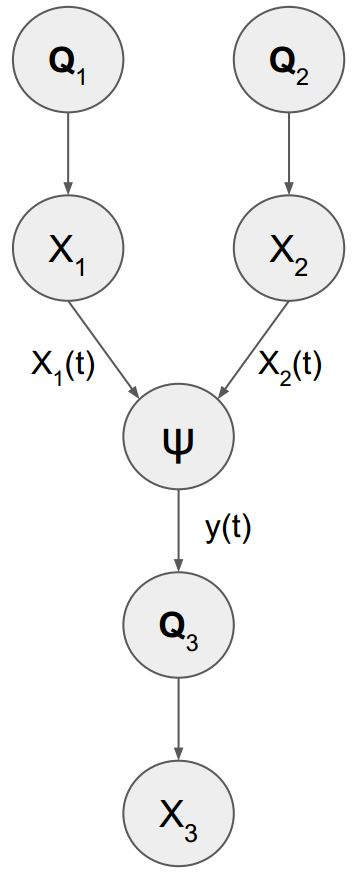
\includegraphics[width=2.5cm]{figures/h_model}
		\caption{Graphical model.}
	\end{center}
	\label{wrap-fig:1}
\end{wrapfigure} 
The communication model considered in this thesis is given in Figure \ref{wrap-fig:1}. The parent nodes, $X_{1}$ and $ X_{2}$, emit messages which carry information about their states. These messages are translated by an observation model, $\psi$, and agent node, $ X_{3} $ makes a decision based on this translated message, $ y $. The main objective is to infer the observation model given the trajectories of nodes.

The messages that are emitted by the parent nodes $X_{1}$ and $ X_{2} $ are modelled as independent homogeneous continuous-time Markov processes $X_{i}(t)$, with state space $ \rchi_{i} = \left\lbrace x_{1}, x_{2}, ..., x_{n} \right\rbrace  $ for $ i \in \left\lbrace 1,2 \right\rbrace $. These processes are defined by transition intensity matrices $ Q_{i} $, where intensities do not depend on time. These matrices are assumed to be gamma distributed.
\begin{equation}
\textbf{Q}_{i} \sim Gam(\alpha_{i}, \beta_{i})\ \ for\ i \in \left\lbrace 1,2\right\rbrace \nonumber
\end{equation}
The agent node does not have a direct access to the messages, but observes a translation of them. The observation model is defined as the likelihood of a translation given the parent messages.
\begin{equation}
\psi \coloneqq p(y(t) \mid X_{1}(t), X_{2}(t))
\end{equation}
The agent  $ X_{3} $ is modelled as inhomogeneous continuous-time Markov process with state space $ \rchi_{3} = \left\lbrace x_{1}, x_{2}, ..., x_{n} \right\rbrace  $, set of actions $ a \in \left\lbrace a_{0}, a_{1}, ..., a_{k}\right\rbrace  $ and set of transition intensity matrices $ \textbf{\textit{Q}}_{3} = \left\lbrace \textbf{Q}_{a_{0}}, \textbf{Q}_{a_{1}}, ..., \textbf{Q}_{a_{k}} \right\rbrace $. 
\begin{equation}
\textbf{Q}_{a} \sim Gam(\alpha_{a}, \beta_{a})
\end{equation}
Given the observation, the agent forms a belief over the parent states, $  b(x_{1}, x_{2}; t) $, that summarizes the past observations.\cite{Kaelbling2011} The policy of the agent, $ \pi(a \mid b) $, is assumed to be shaped by evolution (close) to optimality. Based on the belief state, the agent takes an action, which in the setting described above means to change its internal dynamics through choice of intensity matrix. 

\section{Continuous Time Markov Processes}

A continuous-time Markov process (CTMP) is a continuous-time stochastic process which satisfies Markov property, namely, the probability distribution over the states at a future time is conditionally independent of the past states given the current state.\cite{Cohn2010a} Let X be a CTMP with state space $ \rchi = \left\lbrace x_{1}, x_{2}, ..., x_{n} \right\rbrace  $. Then the Markov property can be written as follows:
\begin{equation}
	\operatorname{Pr}\left(X^{\left(t_{k}\right)}=x_{t_{k}} | X^{\left(t_{k-1}\right)}=x_{t_{k-1}}, \ldots, X^{\left(t_{0}\right)}=x_{t_{0}}\right)=\operatorname{Pr}\left(X^{\left(t_{k}\right)}=x_{t_{k}} | X^{\left(t_{k-1}\right)}=x_{t_{k-1}}\right)
\end{equation}
A CTMP is represented by its transition intensity matrix, $ \textbf{Q} $. In this matrix, the intensity $ q_{i} $ represents the instantaneous probability of leaving state $ x_{i} $ and $ q_{i,j} $ represents the instantaneous probability of switching from state $ x_{i} $ to $ x_{j} $. 
\begin{equation}
	\textbf{Q} = 
	\begin{bmatrix}
	-q_{1} & q_{1,2} & 	{\hdots}  & q_{1,n} \\
	q_{2,1} & -q_{2} & 	{\hdots}  & q_{2,n}  \\
	{\vdots}  & 	{\vdots}  & 	{\ddots}  & {\hdots}  \\
	q_{n,1} &  q_{n,2} &  {\hdots} & -q_{n}
	\end{bmatrix}
\end{equation}
where $ q_{i} = \sum_{i \neq j} q_{i,j}$.\cite{Nodelman1995}

\subsection{Homogenous Continuous Time Markov Processes}
A continuous-time Markov process is time-homogenous when the transition intensities do not depend on time. Let X be a homogenous CTMP, with transition intensity matrix \textbf{Q}. Infinitesimal transition probability from state $ x_{i} $ to $ x_{j} $ in terms of the transition intensities $ q_{i,j} $ can be written as \cite{Cohn2010a}:
\begin{equation}
p_{i,j}(h)=\delta_{ij}+q_{i,j} h+o(h)
\end{equation}
where $ p_{i, j}(t) \equiv Pr(X^{(t+s)}=j\mid X^{(s)}=i) $ are Markov transition functions and o(.) is a function decaying to zero faster than its argument.

The \textit{master equation} is then derived as follows:
\begin{align}
	p_{j}(t) & =\sum_{\forall i} p_{i, j}(h) p_{i}(t-h) \nonumber \\
	\lim_{h\rightarrow 0} p_{j}(t) 
		& = \lim_{h\rightarrow 0} \sum_{\forall i} \left[ \delta_{ij}+q_{i,j} h+o(h)\right]  p_{i}(t-h) \nonumber \\ 
		& = \lim_{h\rightarrow 0} p_{j}(t-h) + \lim_{h\rightarrow 0} h \sum_{\forall i} q_{i,j} p_{i}(t-h) \nonumber \\
	\lim_{h\rightarrow 0} \frac{p_{j}(t) - p_{j}(t-h)}{h} 
		&= \lim_{h\rightarrow 0} \sum_{\forall i} q_{i,j} p_{i}(t-h) \nonumber\\
	\frac{d}{dt} p_{j}(t) & = \sum_{\forall i} q_{i,j} p_{i}(t) \nonumber\\ 
		& = \sum_{\forall i \neq j}\left[  q_{i,j} p_{i}(t) - q_{j,i} p_{j}(t) \right]
	\label{eq:ME}
\end{align}


Eq.\ref{eq:ME} can be written in matrix form:
\begin{equation}
\frac{d}{dt} p = p\textbf{Q}
\end{equation}
The solution to ODE, the time-dependent probability distribution $ p(t) $ is, 
\begin{equation}
p(t)=p(0) \exp (t\textbf{Q})
\end{equation}
with initial distribution $ p(0) $.

The amount of time staying in a state $ x_{i} $ is exponentially distributed with parameter $ q_{i} $. The probability density function $ f $ and cumulative distribution function $ F $ for staying in the state $ x_{i} $ \cite{Nodelman1995}:
\begin{align}
f(t) & = q_{i} \exp \left(-q_{i} t\right), t\geq 0  \label{eq:f(t)_homo}\\
F(t) & = 1 - \exp \left(-q_{i} t\right), t\geq 0 
\end{align}
Given the transitioning from state $ x_{i} $, the probability of landing on state $ x_{j} $ is $ q_{i,j}/q_{i} $.
\subsubsection{Likelihood Function}
Consider a single transition denoted as $ d = <x_{i},x_{j},t> $, where transition occurs from state $ x_{i} $ to $ x_{j} $ after spending t amount of time at state $ x_{i} $. The likelihood of this transition is the product of the probability of having remained at state $ x_{i} $ for that long, and the probability of transitioning to $ x_{j} $.
\begin{equation}
\operatorname{Pr}(d  \mid \textbf{Q}) = \left( q_{i}exp(-q_{i}t) \right) \left( \frac{q_{i,j}}{q_{i}} \right)
\end{equation}
The likelihood of a trajectory sampled from a homogenous CTMC, $ X^{[0,T]} $, can be decomposed as the product of the likelihood of single transitions. The sufficient statistics summarizing this trajectory can be written as $ T[x_{i}] $, total amount of time spent in state $ x_{i} $, $ M[x_{i}, x_{j}] $ total number of transitions from state $ x_{i} $ to $ x_{j} $, we can write down the likelihood of a trajectory $  X^{\left[0,T\right] } $,
\begin{align}
\operatorname{Pr}(X^{[0,T]}  \mid \textbf{Q}) &=  \prod_{d \in X^{[0,T]}} \operatorname{Pr}(d \mid \textbf{Q}) \nonumber\\&=\left(\prod_{ i} q_{i}^{M[x_{i}]} \exp \left(-q_{i} T[x_{i}]\right)\right)\left(\prod_{ i} \prod_{ j \neq i} \left(\frac{q_{i,j}}{q_{i}}\right)^{M\left[x_{i}, x_{j}\right]}\right) \nonumber\\ & = \prod_{i}  exp(-q_{i}T[x_{i}]) \prod_{j \neq i}  q_{i,j}^{M[x_{i},x_{j}]}
\label{eq:lh_traj_homo}
\end{align}
where $ M[x_{i}] = \sum_{j \neq i} M[x_{i}, x_{j}] $ is the total number transitions leaving state $ x_{i} $.

\subsubsection{Marginalized Likelihood Function} 
Let $ X $ be a homogenous CTMP. For convenience, it is assumed to be binary-valued, $ \rchi = \left\lbrace x_{0}, x_{1} \right\rbrace $. The transition intensity matrix can be written in the following form:
\begin{equation}
\textbf{Q} = 
\begin{bmatrix}
-q_{0} & q_{0} \\
q_{1} & -q_{1}
\end{bmatrix}
\end{equation}
where the transition intensities $ q_{0} $ and $ q_{1} $ are gamma-distributed with parameters $ \alpha_{0}$, $ \beta_{0} $ and $ \alpha_{1} $, $ \beta_{1} $, respectively. The marginal likelihood of a sample trajectory $ X^{[0,T]} $ can be written as follows:
\begin{align}
P(X^{[0, T]}) & = \int  P(X^{[0, T]}\mid Q)P(Q) dQ \nonumber\\ & = \int_{0}^{\infty} \left( \prod_{x} \exp(-q_{x}T_{x}) \prod_{x'} q_{xx'}^{M[x, x']}\right) \frac{\beta_{xx'}^{\alpha_{xx'}}{q_{xx'}^{\alpha_{xx'}-1}}\exp(-\beta_{xx'}q_{xx'})}{\Gamma(\alpha_{xx'})} \ dq_{xx'} \nonumber\\ & = \prod_{i\in{0,1}}\int_{0}^{\infty} q_{i}^{M[x_{i}]} \ \exp(-q_{i}T[x_{i}]) \  \frac{\beta_{i}^{\alpha_{i}} \ q_{i}^{\alpha_{i}-1}\ \exp(-\beta_{i}q_{i})}{\Gamma(\alpha_{i})} \ dq_{i} \nonumber\\ & = \prod_{i\in{0,1}} \frac{\beta_{i}^{\alpha_{i}}}{\Gamma(\alpha_{i})} \int_{0}^{\infty} q_{i}^{M[x_{i}] + \alpha_{i} -1} \ \exp(-q_{i}(T[x_{i}]+\beta_{i})) \ dq_{i} \\ & = \prod_{i\in{0,1}} \frac{\beta_{i}^{\alpha_{i}}}{\Gamma(\alpha_{i})} \left( -(T_{i}+\beta_{i})^{M[x_{i}] + \alpha_{i}}\ \Gamma(M[x_{i}] + \alpha_{i}, \ q_{i}(T[x_{i}]+\beta_{i})) \right) \Big|_0^\infty  \\ & = \prod_{i\in{0,1}} \frac{\beta_{i}^{\alpha_{i}}}{\Gamma(\alpha_{i})} \left( (T[x_{i}]+\beta_{i})^{M[x_{i}] + \alpha_{i}}\ \Gamma(M[x_{i}] + \alpha_{i}) \right)
\label{eq:Marg_traj}
\end{align}.
%
%where $ T[x_{i}] $, the amount of time spent in state $ [x_{i}] $, $ M[x_{i},x_{j}] $ the number of transitions from state $ x_{i} $ to $ x_{j} $ and  $ M[x_{i}] = \sum_{i\neq j}M[x_{i},x_{j}] $.\\

%From Eq.11, the integral is solved using computer algebra system WolframAlpha as follows:
%\begin{align}
%\int x^{a} \ \exp(-xb) \ dx = -b^{-a-1} \ \Gamma(a+1, \ bx) + C
%\label{eq:integral}
%\end{align}
%
%Plugging Eq.\ref{eq:Marg_traj} in Eq.\ref{eq:Marg_llh} for both $ X_{1} $ and $ X_{2} $:
%\begin{align}
%\begin{split}
%P(\textit{D} \mid \pi, \Phi ) = P(X_{3}^{[0, T]}\mid Q_{3}^{[0, T]}) \prod_{x_{1}\in{0,1}} \frac{\beta_{x_{1}}^{\alpha_{x_{1}}}}{\Gamma(\alpha_{x_{1}})} \ (T_{x_{1}}+\beta_{x_{1}})^{M_{x_{1}} + \alpha_{x_{1}}}\ \Gamma(M_{x_{1}} + \alpha_{x_{1}})  \\  \prod_{x_{2}\in{0,1}} \frac{\beta_{x_{2}}^{\alpha_{x_{2}}}}{\Gamma(\alpha_{x_{2}})} \ (T_{x_{2}}+\beta_{x_{2}})^{M_{x_{2}} + \alpha_{x_{2}}}\ \Gamma(M_{x_{2}} + \alpha_{x_{2}})
%\label{eq:Marg_llh_final}
%\end{split}
%\end{align}
\subsection{Inhomogeneous Continuous Time Markov Processes}
%In an conventional CTBN, while every node is a Markov process itself, the leaf nodes are \textit{conditional} Markov processes, a type of inhomogeneous Markov process, where the intensities change over time, but not as a function of time rather as a function of parent states. \cite{Nodelman1995} %TODO explain time-dependence in the problem
A continuous-time Markov process is time-inhomogenous when the transition intensities changes over time.
For CTMP, Eq.\ref{eq:f(t)_homo} becomes:
\begin{equation}
f(t) = q_{i}(t) \exp \left(-\int_{0}^{t} q_{i}(u) d u\right)
\end{equation}
\subsubsection{Likelihood Function}
Let X be an inhomogeneous Markov process. $  X^{\left[0,T\right] } $ is a trajectory sampled from this process with $ m $ number of transitions, $ 0 = t_{0} < t_{1} < ... < t_{m} $ are the times where transition occurred, and $ x_{t_{0}}, x_{t_{1}},..., x_{t_{m}} $ are the observed states. The likelihood of trajectory  $  X^{\left[0,T\right] } $ can be written as follows: 
\begin{equation}
L(\textbf{Q}_{X} \colon  X^{\left[0,T\right]} ) = \prod_{k=1}^{m} \left[ q_{x_{k-1}} (t_{k}) \exp \left(-\int_{t_{k-1}}^{t_{k}} q_{x_{k-1}}(u) d u\right) \frac{q_{x_{k-1}, x_{k}} (t_{k})}{q_{x_{k-1}}(t_{k})}\right] 
\label{eq:lh_traj_inhomo}
\end{equation}

%We can formulate our graphical model as $ S = [X, Y, Z] $, where $ Par(Z) = {X,Y} $ and $ Par(X) = Par(Y) =\emptyset $. We can then write the conditional probability:
%\begin{equation}
%\begin{split}
%P\left(S^{\left(t+h\right)}=s' | S^{\left(t\right)}=s\right) = & P\left(X^{\left( t+h\right) }=x' | X^{\left(t\right)}=x, Par(X)^{\left(t\right)}={y,z}\right) \\&  P\left(Y^{\left( t+h\right) }=y' | Y^{\left(t\right)}=y\right) P\left(Z^{\left( t+h\right) }=z' | ^{\left(t\right)}=z\right)
%\end{split} 
%\end{equation}

\section{Belief State in Partially Observable Markov Decision Processes}
As the agent node $ X_{3} $ cannot observe the incoming messages directly, it needs to infer In our problem, cell Z does not have a direct access to its parents' states, rather it observes a summary of them. This is different than observing the states through noisy binary channels, and presents a POMDP problem. Even though it is assumed that the policy of the agent is optimal given the true states of parents, the problem of inferring the observational model remains unsolved and to be addressed.

\subsection{Exact Belief State Update}

In a conventional POMDP, given the \textit{transition function}, $ T(s, a, s^{\prime})$  and \textit{observation function}, $ O(s^{\prime}, a, o) $, the belief state update is computed as follows \cite{Kaelbling2011} \footnote{Since it is assumed that there is no affect of agent $ X_{3} $'s action on the observation or transition function, $ a $ is omitted from the equation.}:
\begin{equation}
\begin{aligned}
b^{\prime}\left(s^{\prime}\right) &=\operatorname{Pr}\left(s^{\prime} | o, a, b\right) =\operatorname{Pr}\left(s^{\prime} | o, b\right) \\
&=\frac{\operatorname{Pr}\left(o | s^{\prime}, b\right) \operatorname{Pr}\left(s^{\prime} | b\right)}{\operatorname{Pr}(o | b)} \\
&=\frac{\operatorname{Pr}\left(o | s^{\prime}\right) \sum_{s \in \mathcal{S}} \operatorname{Pr}\left(s^{\prime} | b, s\right) \operatorname{Pr}(s | b)}{\operatorname{Pr}(o | b)} \\
&=\frac{O\left(s^{\prime}, o\right) \sum_{s \in \mathcal{S}} T\left(s, s^{\prime}\right) b(s)}{\operatorname{Pr}(o | b)}
\end{aligned}
\label{eq:b}
\end{equation}

In Eq.\ref{eq:b}, the transition function is time-independent. However, in our setting, the parent nodes X and Y are modelled as CTMCs with time-dependent transition matrices. 
%To derive \textit{continuous-time belief state}, $ b(t) $, first we need to get the joint transition matrix of X and Y, two independent processes. This operation called \textit{amalgamation} is described in detail by Nodelman \textit{et al} \cite{Nodelman1995}. 
%Let us denote this matrix by $ Q_{XY} $. 
Now we can derive the belief state as follows: 
\begin{equation}
b(x_{1}, x_{2}; t) = P( X_{1}(t) = x_{1},  X_{2}(t) = x_{2}\mid y_{1}, ..., y_{t})
\end{equation}
Denote $ b(t) $, $ t \geq 0 $, as row vector with $ \left\lbrace b(x_{1}, x_{2};t)_{x_{i} \in \rchi_{i}}\right\rbrace  $.
This posterior probability can be described by a system of ODEs
\begin{equation}
\frac{db(t)}{dt} = b(t)\ \textbf{T}
\end{equation}
where the initial condition $ b(0) $ is row vector with $ \left\lbrace P(X_{1}(0)=x_{1}, X_{2}(0)=x_{2})_{x_{i} \in \rchi_{i}}\right\rbrace $ \cite{article}.
\textbf{T} is the joint transition intensity matrix of $ X_{1} $ and $ X_{2} $ and given by amalgamation operation between $ \textbf{Q}_{1} $ and  $ \textbf{Q}_{2} $ \cite{Nodelman1995}.
\begin{equation}
\textbf{T} = \textbf{Q}_{1} * \textbf{Q}_{2}
\end{equation}
The belief update at discrete times of observation $ y_{t} $
\begin{align}
b(x_{1}, x_{2}; t) & = P( X_{1}(t) = x_{1},  X_{2}(t) = x_{2}\mid y_{1}, ..., y_{t}) \nonumber\\ & = \frac{P(y_{1}, ..., y_{t}, X_{1}(t) = x_{1},  X_{2}(t) = x_{2})}{P(y_{1}, ..., y_{t})}  \nonumber\\ & = \frac{P(y_{t} \mid y_{1}, ..., y_{t-1}, X_{1}(t) = x_{1},  X_{2}(t) = x_{2})}{P(y_{t} \mid y_{1}, ..., y_{t-1})} \frac{P(y_{1}, ..., y_{t-1}, X_{1}(t) = x_{1},  X_{2}(t) = x_{2})}{P(y_{1}, ..., y_{t-1})}  \nonumber\\ & = Z_{t}^{-1} \ P(y_{t} \mid x_{1}, x_{2})\ P( X_{1}(t) = x_{1},  X_{2}(t) = x_{2}\mid y_{1}, ..., y_{t-1})  \nonumber\\ & = Z_{t}^{-1}\ {P(y_{t} \mid x_{1}, x_{2})}\ {b(x_{1}, x_{2}; t^{-})}
\end{align}
where $ Z_{t} = \sum_{x_{1}, x_{2}\in X} P(y_{t} \mid x_{1}, x_{2})\ b(x_{1}, x_{2}; t^{-}) $ is the normalization factor \cite{article}.
%
%\begin{equation}
%b_{s^{\prime}}(t) =\frac{\operatorname{Pr}\left(o |s^{\prime}\right) \sum_{s \in \mathcal{S}} \operatorname{Pr}\left(S(t)=s^{\prime} | S(t-h)=s\right) b_{s}(t-h)}{\operatorname{Pr}(o | b)}
%\end{equation}\\
%\begin{equation}
%\begin{aligned}
%\lim_{h\rightarrow 0} b_{s^{\prime}}(t) &= C \lim_{h\rightarrow 0}\left[  \sum_{s \in \mathcal{S}} p_{s, s^{\prime}}(t) b_{s}(t-h)\right]\\
%&= C \lim_{h\rightarrow 0}\left[  \sum_{s \in \mathcal{S}} \left[ \delta_{ss^{\prime}}+q_{s,s^{\prime}} h+o(h)\right]  b_{s}(t-h)\right]\\
%&= C \lim_{h\rightarrow 0}\left[ b_{s^{\prime}}(t-h) + \sum_{s \in \mathcal{S}} q_{s,s^{\prime}} h  b_{s}(t-h)\right]
%\end{aligned}
%\end{equation}
%Due to the scaling factor $ C =\frac{\operatorname{Pr}\left(o |s^{\prime}\right)}{\operatorname{Pr}(o | b)} $, cannot derive $ \frac{d}{dt} b = \textbf{Q}b$, .\\
%However, we can use the conditional distribution of Markov processes as the transition function $ T(s'|s) $ to derive the continuous-time belief state. The conditional distribution over the value of X, a homogenous Markov process, at time t given its value at an earlier time s can be written as 
%\begin{equation}
%\operatorname{Pr}\left(X(t) \mid X(s)\right) = \exp(\textbf{Q}(t-s))
%\end{equation}
%Then the continuous-time belief state becomes:
%\begin{equation}
%b_{s^{\prime}}(t) =\frac{\operatorname{Pr}\left(o |s^{\prime}\right) \sum_{s \in \mathcal{S}}\left[ \exp(\textbf{Q}(h))\right]_{s,s'}  b_{s}(t-h)}{\operatorname{Pr}(o | b)}
%\end{equation}

\subsection{Belief State Update using Particle Filter}

\subsubsection{Marginalized Continuous Time Bayesian Networks}

\subsubsection{Particle Filter}

\section{Likelihood Model of Communication System (?)}